\documentclass[12pt, twoside]{report}
\usepackage[a4paper,bindingoffset=0.2in,%
            left=0.8in,right=0.8in,top=1.2in,bottom=1.2in,%
			]{geometry}
\usepackage{graphicx}
\usepackage{fancyhdr}
\fancyhf{}
\renewcommand{\headrulewidth}{0pt}
\fancyhead[RO,LE]{\thepage}
\pagestyle{fancy}
\setcounter{chapter}{1}
\begin{document}
	\tableofcontents
	
	\newpage
	
% Page no - 5
 
	\chapter{Background and Literature Review}
	\large{The importance of facial expression in social interaction and social intelligence is widely recognized. Facial expression analysis has been an active research topic since 19th century. The first automatic facial expression recognition system was introduced in 1978 by Suwa et al. [83]. This system attempts to analyze facial expressions by tracking the motion of 20 identified spots on an image sequence. Since then, a lot of work has been done in this domain. Various computer systems have been made to help us understand and use this natural form of human communication.}\par
	\large{This chapter reviews the state of the art of what has been done in processing and understanding facial expression. When building an FER system, these main issues must be considered: face detection and alignment, image normalization, feature extraction, and classification. Most of the current work in FER is based on methods that implement these steps sequentially and independently. Before exploring what has been done in literature for implementing these steps, we will briefly describe the problem space for facial expression analysis.}

	\section{Problem Space for Facial Expression Analysis}
	\subsection{Level of Description}
	\large{In general there are two types of method to describe facial expression.}
	
	\newpage
	
% Page no - 6
	\subsubsection{Facial Action Coding System}
	\par 
	\large{The facial action coding system [24] is a human-observer-based system widely used in psychology to describe subtle changes in facial features. FACS consists of 44 action units which are related to contraction of a specific set of facial muscles (Fig.2.1). Some of the action units are shown in Fig.2.2. Conventional, FACS code is manually labeled by trained observers while viewing videotaped facial behavior in slow motion. In recent years, some attempts have been made to do this automatically [69]. The advantage of FACS is its ability to capture the subtlety of facial expression, however FACS itself is purely descriptive and includes no inferential labels. That means in order to get the emotion estimation, the FACS code needs to be converted into the Emotional Facial Action System (EMFACS [28]) or similar systems.}\\

	\begin{figure}[h]%
		\begin{minipage}[t]{.5\textwidth}
    		\centering
    		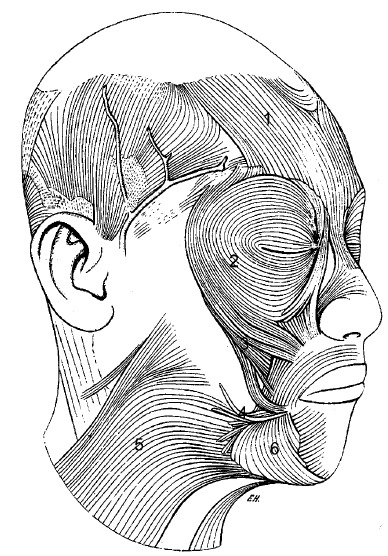
\includegraphics[width=5cm]{img/10_1.jpeg}%
			\caption{Muscles of facial expression. 1,
				frontalis; 2, orbicularis oculi; 3, zygomaticus
				major; 4, risorius; 5, platysma; 6, depressor
				anguli oris [33]}
		\end{minipage}
		\begin{minipage}[t]{.5\textwidth}
    		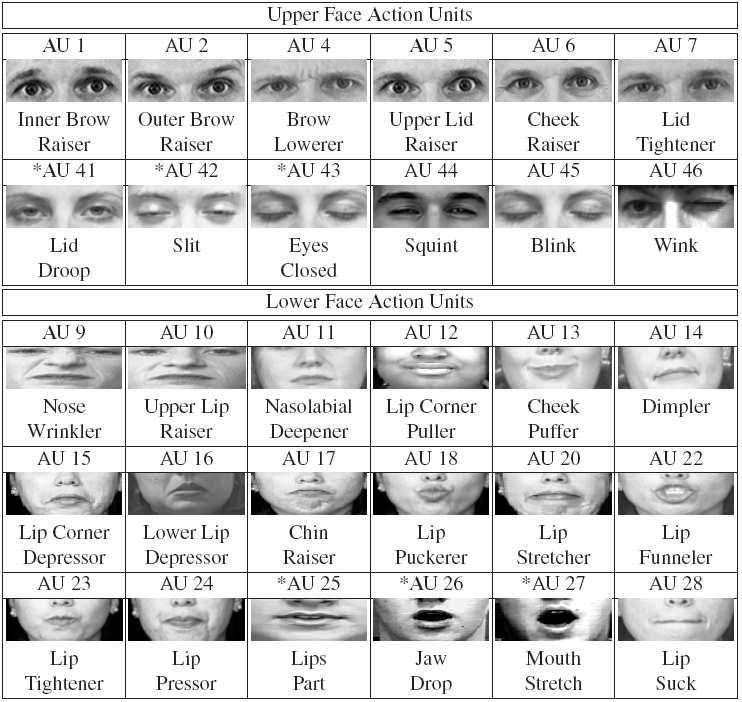
\includegraphics[width=7cm]{img/10_2.jpeg}%
			\centering
			\caption{FACS action units [35]}
		\end{minipage}
		\label{fig:example}%
	\end{figure}

	\newpage
	
% Page no 7
	\subsection*{Prototypic Emotional Expressions}
	Instead of describing the detailed facial features, most FER systems attempt to recognize a small set of prototypic emotional expressions. The most widely-used set is perhaps human universal facial expressions of emotion which consists of six basic expression categories that have been shown to be recognizable across cultures \ref{fig:facialPhenotypes} .

These expressions, or facial configurations have been recognized in people from widely divergent cultural and social backgrounds, and they have been observed even in the faces of individuals born deaf and blind.

These 6 basic emotions, \textit{i.e.}, disgust, fear, joy, surprise, sadness and anger plus ``neutral'' which means no facial expression are considered in this work. Given a facial image, our system either works as a conventional classifier to determine the most likely emotion or estimates the weights (or possibility) of each emotion as a fuzzy classifier does.

	\begin{figure}[h]
    	\centering
    	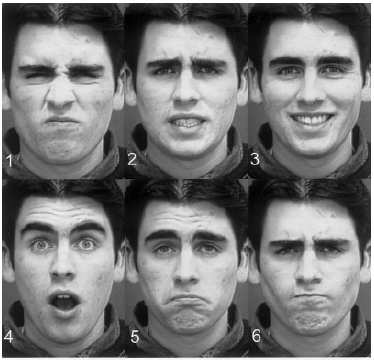
\includegraphics[width=0.5\textwidth]{img/12_1.png}
    	\caption{Basic facial expression phenotypes. 1, disgust; 2, fear; 3, joy; 4, surprise; 5, sadness; 6, anger}
    	\label{fig:facialPhenotypes}
	\end{figure}

	\section{System Structure}
	FER can be considered as a special face recognition system or a module of a face recognition system. So it should be instructive to look at the general architecture of a face recognition system. Normally, it consists of four components as depicted in \ref{fig:processingFlow}

% Page no 8
	\begin{figure}[h]
    	\centering
    	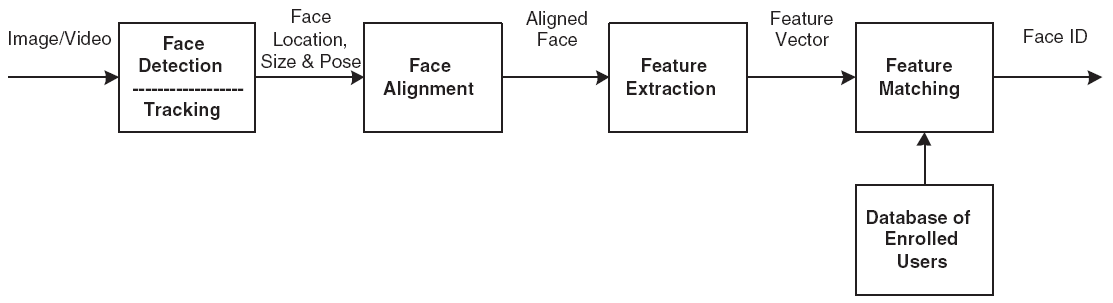
\includegraphics[width=\textwidth]{img/12_2.png}
    	\caption{Face recognition processing flow}
    	\label{fig:processingFlow}
	\end{figure}

	Face detection finds the face areas in the input image. If the input is a video, to be more efficient and also to achieve better robustness, face detection is only performed on key frames and a tracking algorithm is applied on interval frames. Face alignment is very similar to detection, but it is aimed at achieving a more accurate localization. In this step, a set of facial landmarks (facial components), such as eyes, brows and nose, or the facial contour are located; based on that, the face image is rotated, chopped, resized and even warped, this is called geometrical normalization. Usually the face is further normalized with respect to photometrical properties such as illumination and gray scale.

	Feature extraction is performed on a normalized face to provide effective information that should be useful for recognizing and classifying labels in which there is interest, such as identity, gender, or expression. The extracted feature vector is sent to a classifier and compared with the training data to produce a recognition output.

	\section{Face Detection}
	Face detection is the first step in face recognition. It has a major influence on the performance of the entire system. Several cues can be used for face detection, for example, skin color, motion (for videos), facial/head shape, and facial appearance. Most successful face detection algorithms are based on only appearance. This may be because

% Add Page 9 - 22

	\newpage
	
% Page no - 23
	\begin{figure}
		\centering 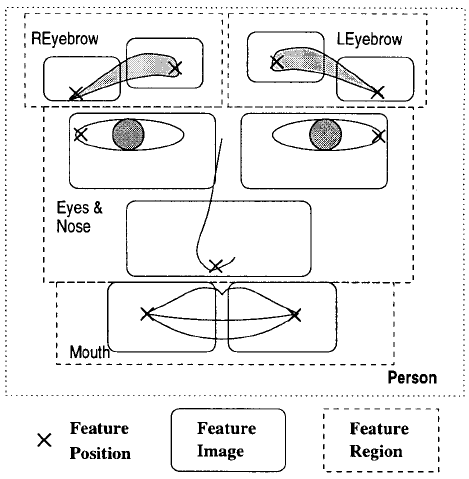
\includegraphics[totalheight=8cm]{img/93_1.png}
		\caption{Figure 2.12: Scheme of the Facial Features and Regions [15]}
		\label{Fig 2.12}
	\end{figure}
	\subsection{Support Vector Machine}
	\large{Support Vector Machine attempts to construct a linear classifier which maximizes the margin between two classes, so it’s also known as Optimal Margin Classifier [9]. Fig.2.13 gives an SVM classifier where $\frac{1}{|w|}$ gives the margin and samples along the hyper-planes are called the support vectors.}
	\par
	\large{It has been proven that SVM minimizes the Structural Risk Function which is considered as a better error estimation than the normallyused Empirical Risk Function in terms of generalization capacity.}
	\par
	\large{We consider data points of the form: $\{(x_1,y_1),...,(x_n,y_n)\}$ where $y_i$ is either 1 or -1, a label denoting the class to which the point $x_i$ belongs. The basic version of SVM can be written as}
	\newline
	\begin{center}
		$argmax\hspace{0.7cm}\frac{1}{||w||}$\\
		$\hspace{4.4cm}s.t.\hspace{0.6cm}y_i(x^Tw-b_0)\ge1,\hspace{0.3cm}\forall i$
	\end{center}
	
	\newpage
% Page no - 24
	\begin{figure}
		\centering 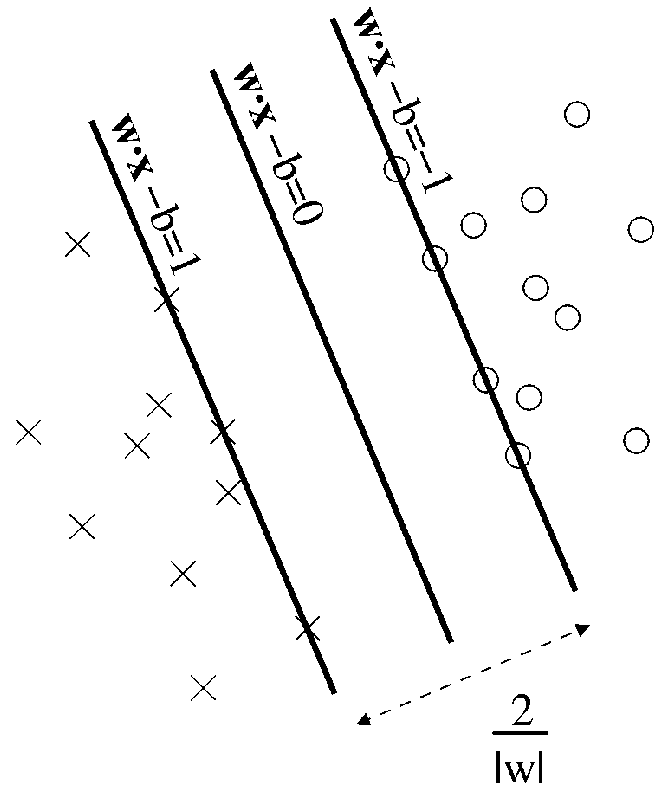
\includegraphics[totalheight=8cm]{img/93_2.png}
		\caption{Figure 2.13: Maximum-margin hyper-planes for a SVM trained with samples from two classes [99]}
		\label{Fig 2.13}
	\end{figure}
	\vspace{0.5cm}
	\large{$||...||$ in (2.27) can be replaced by any distance measure. If norm-2 is used, the problem is equivalent to}
	\begin{center}
		$argmin\hspace{0.7cm}\frac{1}{2}||w||^2$\\
		$\hspace{4.4cm}s.t.\hspace{0.6cm}y_i(x^Tw-b_0)\ge1,\hspace{0.3cm}\forall i$
	\end{center}
	\large{Equation (2.28) is a quadratic programming and according to the strong duality theorem it can be converted to:}
	\begin{center}
		$argmax\hspace{0.7cm}\sum_{i}^{}\alpha_i-\frac{1}{2}\sum_{i}^{}\sum_{j}^{}\alpha_i\alpha_jy_iy_jx^T_ix_j$\\
		$\hspace{-2.5cm}s.t.\hspace{0.6cm}\alpha_i\ge0,\hspace{0.3cm}\forall i$
	\end{center}
	\large{which is called the dual problem of (2.28).In practice, we always use (2.29) as it is easier to handle numerically. Moreover, in (2.29) all the computation of x i is written in terms of inner product, and that means it can be generalized to a nonlinear case by employing Kernel technique.}
		
	\newpage
% Page no - 25		
	\section{Face Database}
	"Because of its non rigidity and complex three-dimensional structure, the appearance of a face is affected by a large number of factors including identity, face pose, illumination, facial expression, age, occlusion, and facial hair. The development of algorithms robust to these variations requires databases of sufficient size that include carefully controlled variations of these factors. Furthermore, common databases are necessary to comparatively evaluate algorithms. Collecting a high quality database is a resource-intensive task: but the availability of public face databases is important for the advancement of the field" [35]. In this section we briefly review some publicly available databases for face recognition, face detection, and facial expression analysis, and we'll mainly focus on the three databases which we will use in this thesis. 
	\par
	To facilitate this statement, we divide face databases into two categories according to their designing goals. In the first part, we'll introduce databases which are normally used for face recognition; those which are dedicated to expression recognition will be discussed in the second part. As only a few databases are of the second type, and FER system shares some common modules with identity recognition system, in this work we also use some databases of the first type.

	\subsection{Databases For Identity Recognition}
	Most face databases are of this category (Table.2.1). To test for robustness, some of them are captured under different poses, illuminations and expressions. However, because they're mainly designed for identity recognition, the expressions are added as noise and usually not well controlled. So in general these databases are considered not suitable for FER research. In our work, we only use them to train peripheral modules (processing and Feature Extraction).

	\section*{The IMM Face Database [66]}
	The IMM Face Database comprises 240 still images of 40 individuals (7 females and 33 males), all without glasses. For each person, 6 images are provided:


	\newpage
% Page no - 26
	\begin{table}
	\caption{Some of the most popular Face Recognition Databases [35] }
	\centering
	\resizebox{14cm}{!}{
		\begin{tabular}{|c||c|c|c|c|}\hline
  			Database & No. of subjects & Pose & Illumination &Facial Expressions\\ \hline\hline
			AR & 116 & 1 & 4 & 4\\\hline
			BANCA & 208 & 1 & ++ & 1\\\hline
			CAS-PEAL & 66-1040 & 21 & 9-15 & 6\\\hline
			CMU HYPER & 54 & 1 & 4 & 1\\\hline
			CMU PIE & 54 & 1 & 4 & 1\\\hline
			Equinox IR & 91 & 1 & 3 & 3\\\hline
			FERET & 1199 & 9-20 & 2 & 2\\\hline
			Harvard RL & 10 & 1 & 77-84 & 1\\\hline
			IMM FACE & 40 & 3 & 2 & 3+\\\hline
			KFDB & 1000 & 7 & 16 & 5\\\hline
			MIT & 15 & 3 & 3 & 1\\\hline
			MPI & 200 & 3 & 3 & 1\\\hline
			ND HID & 300+ & 1 & 3 & 2\\\hline
			NIST MID & 1573 & 2 & 1 & ++\\\hline
			ORL & 10 & 1 & ++ & ++\\\hline
			UMIST & 20 & ++ & 1 & ++\\\hline
			U.Texas & 284 & ++ & 1 & ++\\\hline
			U. Oulu & 125 & 1 & 16 & 1\\\hline
			XM2VTS & 295 & ++ & 1 & ++\\\hline
			Yale & 15 & 1 & 3 & 6\\\hline
			Yale B & 10 & 9 & 64 & 1\\\hline
  
			\hline
		\end{tabular}
  	}
	\label{2.1}
	\end{table}


	\begin{itemize}
		\item Frontal face, neutral expression, diffuse light.
		\item Frontal face, happy expression, diffuse light.
		\item Face rotated approx. 30 degrees to the person’s right, neutral expression, diffuse light.
		\item Face rotated approx. 30 degrees to the person’s left, neutral expression, diffuse light.
	\end{itemize}

	\newpage
	%\onehalfspacing
	
% Page no - 27
	\begin{itemize}
		\item Frontal face, neutral expression, spot light added at the person’s left side.
		\item Frontal face, “joker image” (arbitrary expression), diffuse light.
	\end{itemize}
	\qquad The images are stored in 640 × 480 JPEG files. Owing to technique problems, most images are RGB, but some are grey-scale [66]. One good thing about this database is that manually labeled face contour is available. The following facial structures were annotated using 58 landmarks: eyebrows, eyes, nose, mouth and jaw. These landmarks are divided into seven point paths; three closed and four open as shown in Fig.2.14. In our work, this database will be used to train the ASM and AAM model.
	
	\begin{figure}[h]
		\centering
		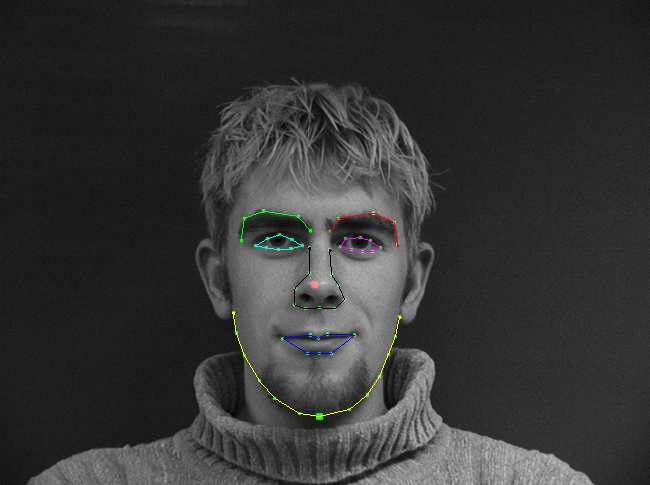
\includegraphics[scale=0.5]{img/98_1.png}
		\caption{Example image from IMM face database}
	\end{figure}
	\vspace{0.5cm}
	\noindent \textbf{CMU Pose, Illumination, and Expression Database [79]} \vspace{0.3cm} \\
	The CMU-PIE database is among the most comprehensive databases in this area. It systematically samples a large number of pose and illumination conditions along with a variety of facial expressions. The PIE database was captured under 21 illuminations (lit by 21 flashes) from 13 directions (using 13 synchronized cameras). In total, there are 41,368 images obtained from 68 individuals. In our experiment, we only use a sub-set of this database which consists of images of 62 people. 25 images were selected for each individual
	
	\pagebreak
	
% Page no - 28	
	\noindent with 5 different viewpoints and 5 different illuminations. Part of the data set is shown in Fig.2.15.
	
	\begin{figure}[h]
		\centering
		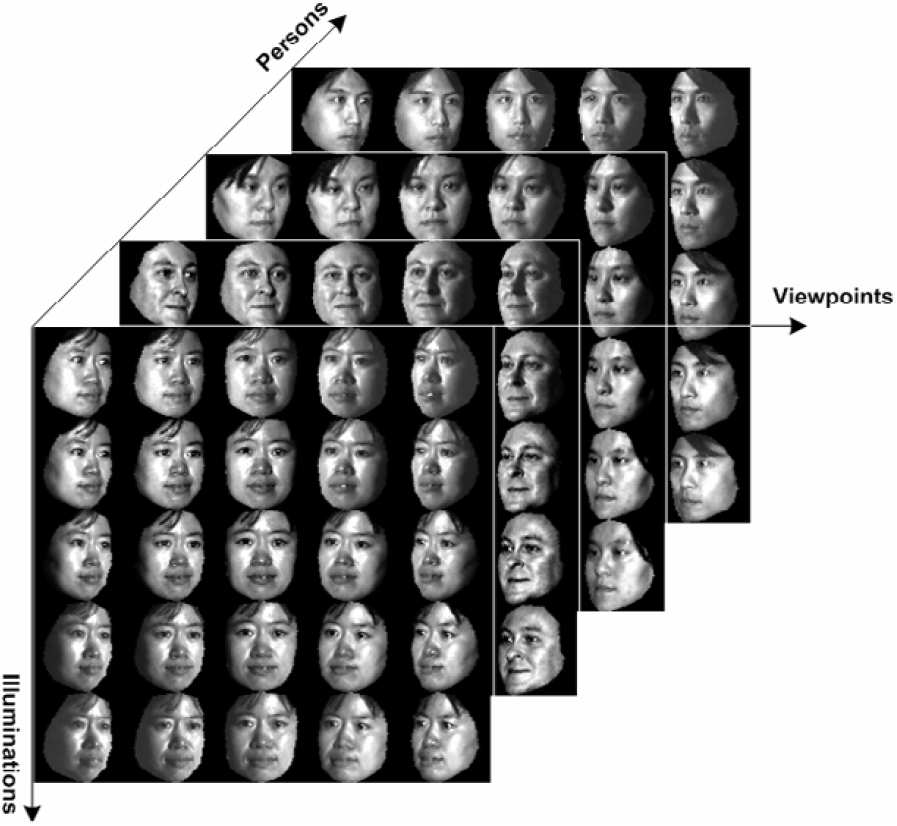
\includegraphics[scale=0.3]{img/98_2.png}
		\caption{A subset of CMU PIE database [53]}
	\end{figure}
	\vspace{0.5cm}
	
	\noindent \textbf{\large \subsection{Databases for Expression Recognition}} \vspace{0.3cm}
	"The human face is able to display an astonishing variety of expressions. Collecting a database that samples this space in a meaningful way is a difficult task" [35]. As a result, there are many fewer databases available for expression recognition (Table 6.1). As mentioned in 2.1.1, there are two ways to describe facial expressions. Available databases can be categorized into two classes according to the description they used. In one group [38] expressions are coded in FACS, while in the other group [57] images are labeled by their sprototypic emotional expressions.
	\vspace{0.1cm} \\
	
	\noindent \textbf{Japanese Female Facial Expression Database [57]}
	\vspace{0.3cm} \\
	The JAFFE database contains 213 images of 10 Japanese female models. Their images are labeled by emotions: six basic emotions (anger, disgust, fear, joy, happy, sad and surprise) are considered and “Neutral” is added as the 7th emotion which is defined through the absence of expression. Fig.2.16 shows example images for one subject along with emotion

	\newpage
	
% Page no - 29
	\begin{table}
		\caption{Commonly used expression recognition databases [35] }
  		\centering
  		\resizebox{14cm}{!}{
  			\begin{tabular}{c||l|c|c|c}
  				Database & No. of subjects & No. of Expressions & 						Image Resolution & Video/Image\\ \hline\hline
  				JAFFE & 10 & 7 & 256 X 256 & Image\\\hline
  				U. Maryland & 40 & 6 & 560 X 240 & Video\\\hline
  				Cohn-Kanade & 100 & 23 & 640 X 480 & Video\\\hline
  			\end{tabular}
  		}
	\end{table}

	labels. The images were originally printed in monochrome and then digitized using a flatbed scanner.
	
	\begin{figure}
		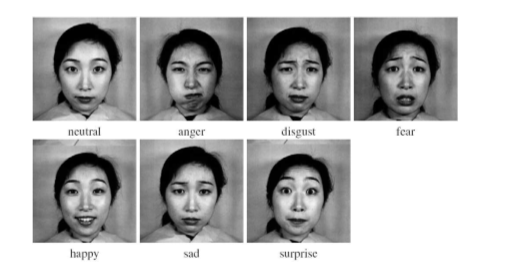
\includegraphics[width=\textwidth]{img/94_1.jpg}
		\caption{Example images from JAFFE database[35]}
		\label{Fig 2.16}
	\end{figure}
	\section{Chapter Summary}
	\par
	In this chapter, we first talked about the background of facial analysis, then gave an overview of the development in this area, and we also briefly introduced some state of the art techniques which might be useful for our system. At the end, we had a glance at some face databases for identity and expression recognition. Starting in the next chapter, we'll discuss the design of our FER system.
	\end{document}

\end{document}